% \documentclass[conference]{IEEEtran}\IEEEoverridecommandlockouts

\documentclass[sigconf]{acmart}

\usepackage{booktabs} % For formal tables


% Copyright
%\setcopyright{none}
%\setcopyright{acmcopyright}
%\setcopyright{acmlicensed}
\setcopyright{rightsretained}
%\setcopyright{usgov}
%\setcopyright{usgovmixed}
%\setcopyright{cagov}
%\setcopyright{cagovmixed}
\newcommand{\psdleq}{\preccurlyeq}
\newcommand{\psdgeq}{\succcurlyeq}

\newcommand{\ourTool}{ToolX}

\newcommand{\Int}{\ensuremath{\mathbb{Z}}}
\newcommand{\Real}{\ensuremath{\mathbb{R}}}

\newcommand{\upperB}{\ensuremath{ub}}
\newcommand{\lowerB}{\ensuremath{lb}}
\newcommand{\target}{\ensuremath{t}}



% DOI
\acmDOI{10.475/123_4}

% ISBN
\acmISBN{123-4567-24-567/08/06}

%Conference
% \acmConference[WOODSTOCK'97]{ACM Woodstock conference}{July 1997}{El
%   Paso, Texas USA}
% \acmYear{1997}

%\setcopyright{usgovmixed}
%\acmConference[DAC '17]{June 18-22, 2017, Austin, TX, USA}
%\acmPrice{\$15.00}
%\acmYear{2017}
%\copyrightyear{2017}
%\acmBadgeL[http://ctuning.org/ae/ppopp2016.html]{ae-logo}
%\acmBadgeR[http://ctuning.org/ae/ppopp2016.html]{ae-logo}
\begin{document}
\title{Synthesizing Safe Timing Bounds for Secure CAN bus in Automotive Applications}


\author{} % for submission



\renewcommand{\shortauthors}{}


\begin{abstract}
% %why ? - platform independent to platform dependent when timing is absent/untrusted
% Timed Automata are a useful tool for modelling platform independent behavior and verifying safety properties of cyber-physical systems, but do not capture the timing behavior of the system running on real hardware. 
% %how ? - use PTA and synthesize the bounds on delays st condition is sat - bounded model checking
% To account for time delays caused by hardware and physical constraints, we use Parametric Timed Automata and synthesize the allowable range of parameters (delays) such that safety properties are still satisfied. 
% %what ? - verify the MaCAN security protocol against safety/timing property  
% We apply this approach to the MaCAN timed security protocol to synthesize bounds on the delays that an implementation may introduce at each step of the protocol, while still preserving some desirable behavior, such as liveness.
%Failure to use off-the-shelf authentication schemes for security of resource constrained vehicular networks has led to the development of custom protocols. To ensure the protocol behaves correctly, formal analysis is performed on a platform independent model. 
%inter-vehicular networks such as
Security issues in the CAN bus have led to the design of custom authentication protocols. To ensure these protocol behave correctly, a platform independent model is developed and formally verified against desired security properties. However, this model fails to capture the timing behaviors of the authentication protocol, which can be violated when it is integrated on a specific platform. As such, we use a platform dependent, parameterized timed automata model of the protocol and synthesize safe delay bounds that will ensure timing behaviors are preserved. We demonstrate feasibility of our approach by synthesizing delay bounds for the MaCAN authentication protocol.           

%However, verification based on platform independent model, fails to check timing behavior of the protocol, which can deviate when the protocol is integrated on a specific platform. 




\end{abstract}


%  purpose of study(why), methodology(how) , results ( what they found) and conclusion (what it means)

%
% The code below should be generated by the tool at
% http://dl.acm.org/ccs.cfm
% Please copy and paste the code instead of the example below. 
%
% We no longer use \terms command
%\terms{Theory}

%\keywords{Autonomous Systems, \LaTeX, text tagging}

%\begin{teaserfigure}
%  \includegraphics[width=\textwidth]{sampleteaser}
%  \caption{This is a teaser}
%  \label{fig:teaser}
%\end{teaserfigure}


\maketitle

\section{Introduction} \label{sec:intro}

%Timed Automoata are a useful tool for modelling cyber-physical systems, but as an abstraction technique, do not capture the exact timing behavior of the implemented system. Existing techniques to integrate implementation details into these models typically require some knowledge of the expected time delays cause by hardware and physical constraints on each transition in the automoata. However, these expected time delays are not always available, or a designer may not want to include the given delays into the trusted base. To address the issue of absent or untrusted timing estimates for an automata modelling a cyber-physical system, use paramaterized 


\textbf{HyperLTL} when traces depend on each other, for example one authentication depends on the authentication of another.

A popular and useful approach to building verified cyber-physical systems (CPS) is to create a platform independent model (PIM) of the intended behaviour of the system. Using this model, various temporal logics can be used to specify and check some properties on that model, such as liveness, deadlock, livelock, etc. While this is an effective method for reasoning on an abstract level, when the CPS is implemented in practice, additional delays are introduced (from hardware and other physical constraints) that are not expressed in the more abstract model. This can lead to models which ensure safety properties that do not hold in practice.

To account for these delays, manufacturers of devices will provide a range of delays that can be expected. These delays can then be integrated into the model to check that saftey properties hold even in the implemented version of the model. 


While manufacturer guarantees can often be taken as safe assumptions, such models are not available in many other situations. For example, when embedding platform independent software into a particular system, the timing model may change based on this hardware. Furthermore, as CPS component development becomes more accessible to individuals, there may not be a central manufacturer that can provide a bounded timing model.

for this reason, we address the inverse problem, where these delays are unknown or untrusted, and the user wishes to discover the acceptable range of delays that will still admit the safety properties of interest.

% A key assumption in verifying time constraints on  embedded cyber physical systems is the that the given timing model is correct. The time for each step between nodes of the automata are given upper and lower timing bounds - usually given by the manufacturer of the device. This expands the trusted base to include the manufacturer.


% Contributions: 
% \begin{itemize}
%     \item Parametric Timed Automata for finding timing constraints of security protocol transitions, given the WCET. 
    
%     \item Showing that the platform independent model is contained within the platform dependent model 
% \end{itemize}



\section{Related Work} \label{sec:related}
%\url{http://phys.org/news/2016-11-scientists-hackers-remotely-cars.html}

As CPS are resource-constrained systems, understanding the impact of any security solutions on  control performance, timing, and resources of the system is important. Furthermore, ensuring the solutions respect the semantic gap between design and implementation is crucial for its correct operation. Consequently, Lin \textit{et al.} \cite{LZV14}, Pasqualetti and Zhu \cite{PZ15} and Zheng \textit{et al.} \cite{ZDRP16} proposed frameworks that analyses the impact of security solutions and consider the gap between controller design and implementation. Lin \textit{et al.} \cite{LZV14} analysed the impact of message authentication mechanism with time-delayed release of keys on real-time constraints of a ground-vehicle. Such a security solution was developed to protect Time Division Multiple Access (TDMA)-based protocol, which is used in many safety-critical systems such as automobile and avionics electronic systems because of their more predictable timing behavior. To ensure the increased latencies (due to delayed key release) did not violate timing requirements, an algorithm to optimize task allocation, priority assignment, network scheduling, and key-release interval length during the mapping process from the functional model to the architectural model, with consideration of the overhead was developed. This algorithm combined simulated annealing with a set of efficient optimization heuristics. However, their approach did not consider the impact of their security solution on sampling periods and control performance. Furthermore, they didn't consider presence of a software platform between the security solution and hardware.     


Pasqualetti and Zhu's \cite{PZ15} method could analyse control performance, security, and end-to-end timing of a resource-constrained CPS under network (cyber) attack that can compromise systems privacy (confidentiality). They have also quantified interdependency between the three system objectives by means of a minimal set of interface variables and relations. In their work, they have considered an adversary that has complete knowledge of the system model and can reconstruct system states from measurements. As a first step, the physical plant was modeled as a continuous time LTI system. The control input was determined using an output-based control law. A relationship was established to show that the control performance improved with reduced sampling time. Next, resiliency of the encryption method, protecting messages transmitted by sensor to controller was evaluated. It was observed that the encryption method increased the sampling period thereby degrading control performance. While implementing the control function on a CPS platform, the end-to-end delay was calculated by incorporating time incurred during sensing, computation, and communication. During development of the scheduling algorithm for the system, it was ensured that the measured delay was within the sampling period. Based on their analysis, they concluded that the control and the security algorithms should be designed based on the implementation platform so as to optimize performance and robustness. 

Zheng \textit{et al.} \cite{ZDRP16} quantify the impact of their security solution on control performance and schedulability. They also analyzed the tradeoffs between security level and control performance while ensuring the resource and real-time constraints were satisfied. For demonstration, a CPS with multiple controllers that share computation and communication resources was considered. A controller, which was modelled as a control task, processed information collected from sensors on a shared resource and commanded actuators to carry out task. To prevent attackers from eavesdropping on the communication medium for obtaining system's internal information, messages from sensors were encrypted. The decryption of these messages were modeled as task. Each of these tasks were given an activation period and worst case execution time. In the system, the control tasks competed for computation resources whereas as messages competed for communication resources. Incorporating the message encryption mechanism introduced resource overhead that impacted schedulability and control performance. To avoid this issue, they framed an optimization problem where control performance (a function of control task period) was the objective function and security level, computation resource, communication resource, and end-to-end latency were constraints. %By varying the security level (function of messages to be encrypted), they ensured that the system achieved optimal control performance and platform schedulability. 




\section{Modeling of Security Protocol for CAN} \label{sec:model}
%TODO:
%why you do the modelling and why synthesis of constraints and why properties? 

In this section, we first describe the \textit{Message authenticated CAN} (MaCAN) protocol \cite{KO15}, which is a broadcast authentication protocol specifically designed for CAN. Then, we briefly describe the \textit{Parametric Timed Automata} framework that we use to model such a protocol.    

\subsection{MaCAN protocol}
%It is backward compatible with deployed technology. 
The MaCAN protocol was designed to increase the security of the standard CAN bus. It enables incorporation of authentication message in CAN frames, which can be verified by either a single or a group of receiving nodes (ECUs). The protocol uses a new partitioning scheme that allows addition of CAN-ID (sender's ECU ID), two flag bits (for distinguishing different message types), and destination node's ID to the traditional CAN frame. The CAN-ID contains six bit source ID (src\_id) that enables the receiving node to identify the sender's node. The flag bits are mapped to the first two most significant bits of the first byte of the data field and rest six bits are used for storing destination node's ID (dst\_id). The remaining seven bytes of the crypt frame data field store the message to be transmitted. The protocol uses different format of messages, details of which can be found in \cite{KO15}.     
\vspace*{-0.15in}
\begin{figure}[h]
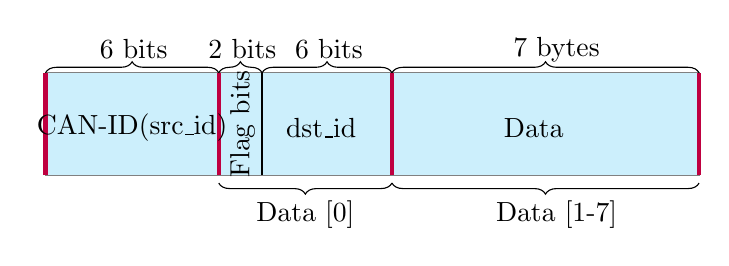
\begin{tikzpicture}
\draw[draw=black!50, fill=cyan!20] (-1, 0.2) rectangle (7.3, 1.5);
\draw [purple,ultra thick] (-1, 0.2) -- (-1,1.5) ;
\draw [purple,ultra thick] (1.2, 0.2) -- (1.2,1.5) ;
\node at (0.1,0.8) {CAN-ID(src\_id)};
\node[rotate=90] at (1.5,0.85) {Flag bits};
\draw [black,thick] (1.75, 0.2) -- (1.75,1.5) ;
\node at (2.5,0.8) {dst\_id};
\draw [purple,ultra thick] (3.4, 0.2) -- (3.4,1.5) ;
\node at (5.2,0.8) {Data};
\draw [purple,ultra thick] (7.3, 0.2) -- (7.3,1.5) ;
\draw [rotate=0,decorate,decoration={brace,amplitude=4pt}]
(-1,1.5) -- (1.2,1.5);
\node at (0.12,1.8) {6 bits};
\draw [rotate=0,decorate,decoration={brace,amplitude=4pt}]
(1.2,1.5) -- (1.75,1.5);
\node at (1.5,1.8) {2 bits};
\draw [rotate=0,decorate,decoration={brace,amplitude=4pt}]
(1.75,1.5) -- (3.4,1.5);
\node at (2.6,1.8) {6 bits};
\draw [rotate=0,decorate,decoration={brace,amplitude=4pt}]
(3.4,1.5) -- (7.3,1.5);
\node at (5.49,1.8) {7 bytes};
\draw [decorate,decoration={brace,mirror,amplitude=4pt}]
(3.4,0.1) -- (7.3,0.1);
\node at (5.49,-0.3) {Data [1-7]};%  %% Grid lines 
\draw [decorate,decoration={brace,mirror,,amplitude=4pt}]
(1.2,0.1) -- (3.4,0.1);
\node at (2.3,-0.3) {Data [0]};
%     \draw[help lines] (-1, -1) grid (7.3, 1);
%   \foreach \i in {-1,...,7} {
%         \node[anchor=north] at(\i, -1) {\footnotesize \i};
%     }
%     \foreach \i in {-1, ...,1} {
%         \node[anchor=east] at (-1, \i) {\footnotesize \i};
%     }
\end{tikzpicture}
\vspace*{-0.1in}
\caption{Crypt Frame} \label{fig:cframe}
\end{figure}
\vspace*{-0.15in}

The MaCAN protocol requires a \textit{key server} (KS) for distributing key among the nodes and a \textit{time server} (TS) to synchronize internal counter of nodes with the global time. The KS maintains the session keys and stores the symmetric long-term keys (LTK) of all the nodes (ECUs) of the vehicle network. The TS periodically provide precise time to all the nodes and respond to authenticated time request. With this setup, the protocol performs three procedures: (i) session key establishment, (ii) signal authentication, and (iii) time synchronization, for secure message transmission in CAN network.               

\vspace*{0.1in}
\noindent \underline{\textit{Session Key Establishment}}

\vspace*{0.05in}
Prior to the exchange of authenticated messages among ECUs (nodes), the MaCAN protocol requires the sender ($ECU_i$) and the receiver ($ECU_j$) nodes to obtain a session key by communicating with the \textit{key server}. Figure. \ref{fig:skest} illustrates the key establishment procedure. To send the session keys to the nodes, the \textit{key server} uses the stored LTK of ($ECU_i$) and ($ECU_j$).

The procedure starts with $ECU_i$ sending a challenge $C_i$ and ID $id_j$ of the node it wants to communicate with to the \textit{KS} (\ref{ske1}). The \textit{KS} respond by sending \textbf{SK} message that contain the fresh session key $SK_{ij}$, the challenge $C_i$, and IDs of $ECU_i$ ($id_i$) and $ECU_j$ ($id_j$), encrypted with the LTK $K_{i, LTK}$ of $ECU_i$ (\ref{ske2}). Subsequently, \textit{KS} sends
a request for challenge (\textbf{RC}) to $ECU_j$, notifying it of the session key that has been generated (\ref{ske3}). After $ECU_i$ decrypts the session key $SK_{ij}$ and verify the challenge value, it sends an acknowledgement message \textbf{ACK} to $ECU_j$. The \textbf{ACK} message consist of a 24-bit group field $gf$ that indicates the nodes the sender ($ECU_i$) is aware of being authenticated and a signed (with $SK_{ij}$) cipher based message authentication code (\textit{cmac}) that includes the current timestamp $T$, the group field, and ID of $ECU_j$ (\ref{ske4}). Subsequently, $ECU_j$ follows an analogous procedure to obtain the session key from the key server and notify $ECU_i$ (\ref{ske5}, \ref{ske6}, \ref{ske7}). When $ECU_i$ verifies the authenticity of the \textbf{ACK} message received from $ECU_j$ and does not find its ID in the group field, it sends another \textbf{ACK} to $ECU_j$ with both $id_i$ and $id_j$ bits in the group field set (\ref{ske8}).     
%informing it of the received session key
\vspace*{-0.15in}
\begin{figure}[h]
\begin{align}
 ECU_i \rightarrow KS &: \mathbf{CH}, C_i, id_j \label{ske1}\\ 
 KS \rightarrow ECU_i &: \mathbf{SK}, \{C_i, id_j, id_i, SK_{ij}\}_{K_{i,LTK}} \label{ske2}\\
 KS \rightarrow ECU_j &: \mathbf{RC}, id_i \label{ske3}\\ 
 ECU_i \rightarrow ECU_j &: \mathbf{ACK}, gf(id_i),\{cmac(T, id_j, gf(id_i))\}_{SK_{ij}} \label{ske4}\\
 ECU_j \rightarrow KS &: \mathbf{CH}, C_j, id_i \label{ske5}\\
 KS \rightarrow ECU_j &: \mathbf{SK}, \{C_j, id_j, id_i, SK_{ij}\}_{K_{j,LTK}} \label{ske6}\\
ECU_j \rightarrow ECU_i &: \mathbf{ACK}, gf(id_j), \{cmac(T, id_i, gf(id_j))\}_{SK_{ij}} \label{ske7}\\
ECU_i \rightarrow ECU_j &: \mathbf{ACK}, gf(id_i|id_j), \{cmac(T, id_j, gf(id_i|id_j))\}_{SK_{ij}} \label{ske8}
\end{align}
\vspace*{-0.2in}
\caption{MaCAN session key establishment procedure} \label{fig:skest}
\end{figure}

\vspace*{-0.1in}
The MaCAN protocol supports authentication of groups with more than two ECUs. The groups are formed by members with same trust level (e.g. ECUs made by the same manufacturer can form a group) and they share the same session key for message exchange.    

\vspace*{0.1in}
\noindent \underline{\textit{Signal Authentication}}

\vspace*{0.05in}
After establishing the session keys, the ECUs communicate with each other by periodically exchanging messages with signal values (e.g. sensor data of tire pressure is a signal). To receive a signal $sig\#$, the receiving node $ECU_i$ should first send an authenticated signal request $\mathbf{SIG\_AUTH\_REQ}$ message to node $ECU_j$ (\ref{sa1}). The request message is a signed $cmac$ that includes the signal number $sig\#$ that needs to be authenticated, \textit{presc} that specifies the signing behavior ($presc =0$: request the next message to be authenticated, $presc =1$: request each following message to be authenticated), the current time stamp $T$, and the sender and receiver node's IDs. After verifying the $cmac$, $ECU_j$ sends the $\mathbf{AUTH\_SIG}$ message that contains the signed signal value $Signal$ to $ECU_i$ (\ref{sa2}).                  

\vspace*{-0.15in}
\begin{figure}[ht]
\begin{align}
 ECU_i \rightarrow ECU_j &: \mathbf{SIG\_AUTH\_REQ}, sig\#, presc, \nonumber \\ 
                         &\{cmac(T, id_i, id_j, sig\#, presc)\}_{SK_{ij}} \label{sa1}\\
 ECU_j \rightarrow ECU_i &: \mathbf{AUTH\_SIG}, sig\#, Signal, \nonumber \label{sa2}\\ 
                         &\{cmac(T, id_i, id_j, sig\#, Signal)\}_{SK_{ij}} 
\end{align}
\vspace*{-0.2in}
\caption{MaCAN signal authentication procedure} \label{fig:sauth}
\end{figure}

\vspace*{-0.1in}
\noindent \underline{\textit{Time Synchronization}} 

\vspace*{0.05in}
The ECUs of the MaCAN protocol uses time $T$ as one of the inputs in the $cmac$ function. As such, each ECU has an internal clock that is synchronized to the global clock of the \textit{time server (TS)}. The global time is broadcasted periodically in an unauthenticated form by the $TS$. Every ECU receives the time signal and compare it against its internal clock value. If there is a large mismatch between the time values, then the ECU request $TS$ for an authentic time value by sending a challenge message $\mathbf{CH}$ with $fwd\_id$ set to $0$ and the challenge $C_i$ (\ref{tau1}). Subsequently, the $TS$ responds with the authenticated time $\mathbf{AT}$ message, which is signed with the ECU's session key $SK_{ij}$ and contains the last broadcasted timestamp value $T$ and the challenge $C_i$ (\ref{tau2}).                  

\vspace*{-0.15in}
\begin{figure}[ht]
\begin{align}
 ECU_i \rightarrow TS &: \mathbf{CH}, C_i, fwd\_id = 0 \label{tau1} \\ 
 TS \rightarrow ECU_i &: \mathbf{AT}, T, \{cmac(T, C_i)\}_{SK_{i,TS}} \label{tau2}
\end{align}
\vspace*{-0.2in}
\caption{MaCAN time synchronization procedure} \label{fig:tauth}
\end{figure}

\vspace*{-0.1in}
As each communication signal (or message) of the network uses the current time value, attack such as replay can be detected and ECUs can be prevented from being affected by corrupted messages. 

\subsection{Modeling of Security Protocol}

% To ascertain the MaCAN protocol abide by the timing properties of the vehicle network, we first model the protocol using the formalism of \textit{Parametric Timed Automata}, which is an extension of the class of Timed Automata. Then, we find the bounds on the parameters   
Next, we use the formalism of \textit{Parametric Timed Automata} (PTA), which is an extension of the class of Timed Automata (TA) to model the protocol ~\cite{BBHBC14}. Unlike TA that uses \textit{constants} in the clock constraints, the PTA allow use of \textit{parameters} i.e. unknown constants within these constraints.

\begin{definition}
A \textit{PTA} is a tuple of the form $\mathcal{M} = (\Sigma, L, l_0, X, P, I, E, K)$, where $i) \; \Sigma$ is a finite set of actions, $ii) \; L$ is a finite set of locations, $iii) \;l_0 \in L$ is the initial location, $iv) \; X$ is a finite set of non-negative real valued $\mathbb{R}^+$ clocks, $v)\; P$ is a finite set of $\mathbb{R}^+$ parameters, $vi)\; I$ is the invariant that assign a guard  $g(X)$ - constraint over $(X, P)$ of the form $x \sim p$, where $\sim \, \in \{ <, \leq, \geq , > \}$ - to every $l \in L$, $vii) \;E$ is a set of edges $e = (l, g, a, R, l')$ where $l, l' \in L$ are the source and destination locations, $a \in \Sigma$, $g$ is a guard, and $R \subseteq X$ is a set of clocks to be reset, and $viii) \;K$ is a constraint over $P$.    
\end{definition}

\raj{Implement the model in IMITATOR}
% relate the PTA to the security protocol. 
% assumptions while modeling the protocol such as use of counter for timeouts between transition and action to take when timeout.
% assumption : we have the platform independent model 

\section{Side Channel Attack} \label{sec:property}
\raj{Write down the attack model for the protocol}


%\section{Methodology} \label{sec:method}
%
% \textbf{Goal of Project}

% Given a CPS platform and application SW, how can we find timing bounds which are extensible i.e. evolution or modification of the system doesn't effect the timing bounds. 

% A key assumption in verifying time constraints on  embedded cyber physical systems is the that the given timing model is correct.
% The time for each step between nodes of the automata are given upper and lower timing bounds - usually given by the manufacturer of the device.
% This expands the trusted base to include the manufacturer.

% While manufacturer guarantees can often be taken as safe assumptions, such models are not available in many other situations.
% For example, when embedding platform independent software into a particular system, the timing model may change based on this hardware.
% Furthermore, as cyber physical system component development becomes more accessible to individuals, there may not be a central manufacturer that can provide a bounded timing model.

\subsection{Motivations}

1) cant trust the manufacture

2) the manufacturer things could be hacked, and we want to know 'how can the timing guarantees from the manufacture be hacked' so that we still have a safe/stable system.


\textbf{Outline of approach}

\begin{enumerate}
    \item Derive average timing bounds for each atomic step of the CPS through simulation.
    \item To safely generalize the simulation Assume a probabilistic distribution over the simulation time to get bounds.
    \item Using a model checker, find the minimal distribution that implies bounds on the timing model such that the system still satisfies the safety conditions.
\end{enumerate}


\iffalse

http://adt.cs.upb.de/timmo-2-use/publications.htm

http://ieeexplore.ieee.org/abstract/document/7927248/

http://dl.acm.org/citation.cfm?id=2883827

http://jin.ece.ufl.edu/papers/ISVLSI16_CPS.pdf

\fi
% How are timing model/ constraints derived in vehicles? 

































%\textit{Informal Definition of Problem:}

%\begin{itemize}
%    \item 1. Impact of 
%\end{itemize}

% Understanding the impact of security solutions on performance, timing, and resources of the system is essential for its effective operation. Effecting the performance of a real-time resource-constrained CPS could result in undesired consequence. As such we intend to develop a framework that can analyze the impact of security solutions on design metrics of the system. In our framework, we model the system architecture of CPS using platform-based design methodology \cite{SDP12}. The design requirements such as performance, timing, resource along with security are represented as \textit{contracts}. A \textit{contract} is a pair $\mathcal{C} = (A, G)$ of $\{$Assumptions, Guarantee$\}$ of properties that must be satisfied by the set of all inputs and all outputs to the system. We use \textit{quantitative model checking} technique to verify the system against these contracts \cite{GS04}. In this approach, a model $\mathcal{M}$ of a system with an initial state \verb"s"$_{0}$ is expressed as a discrete or continuous time Markov chain, contracts, $\varphi$, are represented using a specification language such as Linear Temporal Logic. Using these notations, the model checking problem can be formally stated as $\mathcal{M},$ \verb"s"$_0 \models \varphi $. %\sim p$ iff $\mathbb{P}_{\mathcal{M}^*} (\underset{\sigma \in Act}{\bigcup} \pi (s_0, \sigma o_\varphi)) \sim p$ .
% %, $p \in [0,1]$ is a probability threshold, and $\bowtie \, \in \{ > , < , \geq, \leq \}$.
% While verifying the system, it should be ensured that the contracts are satisfied within some user defined probability bound. Based on results of the verification process, we can quantify the impact of the design metrics on the system. If the system satisfies all the contracts, we can \textit{certify} the security solution to be appropriate for the system.

% New Ideas

% Resource managment while under attack

% in the case of V2V communications, can the bandwidth be overloaded?
% If a resource is being over utilized in a way consistent with an attack, do a \textit{soft restart} of that resource.
% Wipe the memory, but not the whole system, in order to return to a safe uncompromized state. 
% Need to then show that the default operation after wiping a resource will keep the system in the stable region long enough for the particular resource to recover normal operations.

% Also, a paper on safe restarts\cite{abdi2017application}.




\section{Parameter Bound Synthesis}
 
The \textit{bounded integer parameter synthesis problem} from~\cite{DBLP:journals/corr/BezdekBHBC14}, is defined as follows:
Given a parametric timed automaton $\mathcal{M}$, a labeling function $\mathcal{L}$, an LTL property (verification condition) $\phi$, a lower bound function $\lowerB: P \to \Int$ and an upper bound function $\upperB: P \to \Int $, 
  compute the set of all parameter valuations $v: P \to \Int$ such that 
\begin{align*}
  &\lowerB(p) < v(p) < \upperB(p) \land \\
  &(M,v,L) \models \phi
\end{align*}

However, in the context of embedded systems, the bounds $\lowerB$ and $\upperB$ must be taken from the manufacturer.
If the manufacturer is not able to provide such bounds, or we do not want to take these as an assumptions, we need to synthesize these bounds instead.

For this reason, we formulate the \textit{parameter bound synthesis problem}, where the goal is to find upper and lower bounds such that all valuations within those bounds satisfy the verification condition.
In the CPS domain, this corresponds to the question ``what are the most flexible bounds on the delay my system can induce, such that the overall system is safe?''
Formally, given a parametric timed automaton $\mathcal{M}$, a labeling function $\mathcal{L}$, an LTL property $\phi$, and a target valuation function $\target(p): P \to \Real$,
find the lower bound $\lowerB: P \to \Real$ and upper bound $\upperB : P \to \Real$ functions such that 
%
\begin{align*}
  &\lowerB(p) \leq \target(p) \leq \upperB(p) \land \\ 
  &\forall v.\ \lowerB(p) < v(p) < \upperB(p).\ (M, v,L) \models \phi
\end{align*}
%
subject to the linear optimization/maximization condition 
\begin{align*}
\text{max}(\mathcal{OP}(\lowerB,\upperB,t))
\end{align*}

We leave the exact optimization condition (definition of flexible bounds) up to the user, as certain use cases may call for slightly different system needs.
For example, if the implementation of our system induces a large range for every parameter, we may seek to maximize the minimum range of the bounds.
This finds gives us the most relaxed condition on the bounds so that, if our implementation can meet those bounds, the system is still safe.
%
\begin{align*}
	\mathcal{OP}(\lowerB,\upperB,t) = \text{min}(\upperB(p) - \lowerB(p))
\end{align*}
%
It may be the case that we find that the bounds are too tight for the system implementation to guarantee. 
In this case, we may seek another another optimization condition, that satisfies the verification condition and is possible for the implementation to guarantee.
For example, our implementation may be able to guarantee that sum of the upper bounds will be less than some value.
\begin{align*}
\mathcal{OP}(\lowerB,\upperB,t) = \Sigma_{p} \ \upperB(p)
\end{align*}
%
In a sense, the optimization function $\mathcal{OP}$ is an analog to finding the weakest precondition.
The larger the value of the $\mathcal{OP}$, the more system implementations will satisfy the verification condition.
We enforce the restriction here that it is always a maximization problem, and the $\mathcal{OP}$ is always linear (TODO is this necessary?).

\subsection{Decidability}

This problem can be framed as a decision problem in two different ways.
First, as a general optimization, ``Does there exist a global maximum value for which all valuations within the bounds satisfy $\phi$?''.
This problem is undecidable, as we can reduce this to the unbounded integer parameter synthesis problem, which is known to be undecidable~\cite{benevs2015language}.
TODO proof - actually im not sure about this, even over integers.

Second, we can frame the problem as ``Does there exist a global maximum value less than $k$ for which all valuations within the bounds satisfy $\phi$?''
This seems decidable for integers, as we could enumerate every \lowerB and \upperB, and check each valuation within those bounds.
Th complexity of LTL model checking is exponential in the size of the spec.
There are only finitely many options for \lowerB and \upperB, since \lowerB is finitely bounded by $\forall p. 0 \leq \lowerB(p) \leq \target(p)$.




% The continuous-time plant in presence of noise and attack on output:
% \begin{align}
%     \dot{x}_p &= f_p(x_p, \hat{u}) + w_p \qquad y = g_p(x_p, \eta (t)) + v_p 
% \end{align}

% where, $x_p \in \mathbb{R}^{n_p}$ represents the state of the plant, $\hat{u} \in \mathbb{R}^{n_u}$ represents the control values implemented at the plant, $w_p \sim N(0, Q)$ is the additive zero mean Gaussian noise, $y \in \mathbb{R}^{n_y}$ is the output of the plant, $v_p \sim N(0, R)$ is the additive zero mean Gaussian measurement noise, and $\eta (t)$ is the variable for attack on sensor. During attack, $\eta (t)$ corrupts the output of the plant ($y$), which is measured by sensors. 


% The plant is controlled by a controller over the shared communication network, whose equations are:
% \begin{align}
%     \dot{x}_c &= f_c(x_c, \hat{y}) \qquad u = g_c(x_c, \hat{y}, \mu (t)) 
% \end{align}

% where, $x_c \in \mathbb{R}^{n_c}$ represents the state of the controller,  $\hat{y} \in \mathbb{R}^{n_y}$ is the most recent output (either good or corrupted by attack) of the plant available to the controller, $u \in \mathbb{R}^{n_u}$ represents the controller output, and $\mu (t)$ is the variable for attack on actuator. The controller output ($u$) can be manipulated by cyber or physical attack, which is represented by $\mu (t)$. Due to the presence of communication network, $u \neq \hat{u}$ and $y \neq \hat{y}$. In this setup, sensors are time-driven and both actuator and controller are event-driven. As the controllers, sensors, and actuators are connected via a shared network, they are s\upperBject to varying transmission intervals and varying delays. Due to varying transmission intervals, the instants ($t_k \in \mathbb{R}_{\geq 0}, \; k \in \mathbb{N}$) at which the plant outputs and control values are sampled and transmitted over network are non-equidistantly spaced in time. These transmitted values are received by other units in the network after a delay of $\tau_k \in \mathbb{R}_{\geq 0}$, with $\tau_k \in [\tau_{min}, \tau_{max}]$, for all $k \in \mathbb{N}$. This delay is due to the speed at which data travels in the network and it should be less than transmission interval to ensure correct operation of the controllers. In NCS, a scheduling protocol is used in the network to ensure data from all sensors and actuators are not transmitted at the same time. Moreover, while updating the values of $\hat{y}$ and $\hat{u}$, the network is assumed to operate in a zero-order-hold (ZOH) manner i.e. these values remain constant while being updated. 


% TODO - find a formal model to embed the above equations into some logical formula that can be checked (with wieghted max-smt?).
% We want to know, given a single scheduler (instance of the model), how much delay must be introduced to inalidate the saftey/stability specifications of the system. If the attacker can only introduce delay at one point (step) in the system, how much delay must be introduced. If the attacker can introduce a global delay, how much is needed? What about s\upperBsets of modules (steps in system).


\section{Evaluation}

To test our algorithm, we built a tool, \ourTool, and tested it on real-world case studies from the CPS domain.


%\section{Estimation of Optimal Bounds} \label{sec:method}
%\input{secs/boundest}

% \section{Case Study} \label{sec:demo}
% \input{secs/5-results}


% \section{Conclusion} \label{sec:conclude}
% \input{secs/6-conclusion}

% \section{Notes}\label{sec:notes}
% \begin{itemize}
    \item Extensive form is tree based representation of turn based games. Imperfect information in turn based or sequential game means one player cannot determine the choice to be made by the other player because both the choices are equally likely. Ex: there are two  nodes of player 1 from the two branches of player 2 and in the next move player 2 doesn't know which branch player 1 will select. Ex: Prisoners dilemma in extensive form. 

    \item A normal form game can be trivially transformed into an equivalent imperfect-information game. 
\end{itemize}

% \pagebreak
\bibliographystyle{ACM-Reference-Format}
\bibliography{cps}
\end{document}




%********************************* ROUGH ****************************************************


% \author{\IEEEauthorblockN{Raj Gautam Dutta, Xiaolong Guo, and Yier Jin}
% \IEEEauthorblockA{Department of Electrical and Computer Engineering,
% University of Central Florida}
% \textit{rajgautamdutta@knights.ucf.edu, guoxiaolong@knights.ucf.edu, yier.jin@eecs.ucf.edu}
% }

%\author{\IEEEauthorblockN{
%Raj Gautam Dutta%\IEEEauthorrefmark{}
%, Xiaolong Guo%\IEEEauthorrefmark{}
%, and Yier Jin%\IEEEauthorrefmark{}
%\\
%\IEEEauthorblockA{%\IEEEauthorrefmark{}
%Department of Electrical and Computer Engineering, University of Central Florida}}%}\vspace{-0.2in}
%\{rajgautamdutta, guoxiaolong\}@knights.ucf.edu, yier.jin@eecs.ucf.edu
%\vspace{-0.15in}} % for submission

% \author{\IEEEauthorblockN{Raj Gautam Dutta}
% \IEEEauthorblockA{Department of Electrical and\\Computer Engineering\\
% University of Central Florida\\
% Orlando, FL 32816-2362\\
% Email: rajgautamdutta@knights.ucf.edu}
% \and
% \IEEEauthorblockN{Xiaolong Guo}
% \IEEEauthorblockA{Department of Electrical and\\Computer Engineering\\
% University of Central Florida\\
% Orlando, FL 32816-2362\\
% Email: guoxiaolong@knights.ucf.edu}
% \and
% \IEEEauthorblockN{Yier Jin}
% \IEEEauthorblockA{Department of Electrical and\\Computer Engineering\\
% University of Central Florida\\
% Orlando, FL 32816-2362\\
% Email: yier.jin@eecs.ucf.edu}}
